\documentclass[11pt,a4paper]{article}

\usepackage[margin=1in]{geometry}
\usepackage{amsmath,amssymb,amsthm}
\usepackage{booktabs}
\usepackage{graphicx}
\usepackage{float}
\usepackage{microtype}
\usepackage{parskip}
\usepackage[colorlinks=true,linkcolor=black,citecolor=black,urlcolor=black]{hyperref}

\newtheorem{proposition}{Proposition}[section]
\newtheorem{theorem}[proposition]{Theorem}
\theoremstyle{definition}
\newtheorem{definition}[proposition]{Definition}
\theoremstyle{remark}
\newtheorem{remark}[proposition]{Remark}

\newcommand{\logmap}{f_r}
\newcommand{\R}{\mathbb{R}}
\newcommand{\PF}{\mathcal{L}}

\title{Chaos and Invariant Measures in the Logistic Map:\\
       from Fixed Points to a Markov Coarse-Graining}
\author{{Arjun Sharma}}
\date{\today}

\begin{document}

\maketitle

\begin{abstract}
\noindent
This is a study of the logistic map, a single quadratic recurrence with one
tunable parameter, and one of the simplest systems capable of chaos. As the
parameter increases, the map passes from a stable fixed point through a
cascade of period doublings into chaotic behaviour, and it does so with a
structure that is universal across a wide class of unrelated systems. The work
follows that route quantitatively: deriving the fixed points and their
stability condition analytically and confirming both numerically, extracting
the Feigenbaum constant from the cascade, measuring the rate of separation of
nearby orbits, and characterising the long-run statistics of a chaotic orbit
both in closed form and by coarse-graining the map into a Markov chain, whose
stationary distribution is shown to converge towards that closed form under
refinement of the partition. The coarse-graining is carried out twice, once
with the transition matrix built exactly from the map and once with it
estimated from a single trajectory, and the two constructions behave in
opposite ways under refinement. That contrast, rather than any individual
agreement, is the main finding reported here.
\end{abstract}

\tableofcontents

\bigskip

\section{Introduction}

\subsection{The map}

The logistic map is the recursion
\begin{equation}
  x_{n+1} = \logmap(x_n), \qquad \logmap(x) = r\,x(1-x),
  \label{eq:map}
\end{equation}
with a single real parameter $r$. It was introduced as a population model, in
which $x_n$ is a population expressed as a fraction of a carrying capacity,
$r$ is a growth rate, and the factor $(1-x_n)$ suppresses growth as the
population saturates. Its interest is that a rule involving one multiplication
and one subtraction produces behaviour ranging from convergence to a single
steady state, through cycles of period two, four and eight, to motion that is
aperiodic and unpredictable in a precise sense \cite{May1976}.

The tension that makes the map worth studying numerically is this. The
dynamics are deterministic, so $x_0$ fixes the entire orbit. Yet in the
chaotic regime the orbit is so sensitive to $x_0$ that no finite-precision
computation can track it for more than a few dozen steps, while the long-run
statistics of the orbit, meaning the fraction of time it spends in each part
of the interval, are stable, reproducible and available in closed form. The
natural objects of study are therefore not individual trajectories but the
invariant measure describing where trajectories spend their time, and the
Lyapunov exponent quantifying how fast nearby trajectories separate.

\subsection{Structure and method}

The organising principle is that wherever an exact result is available it is
derived first and then used as a test, and only afterwards are the quantities
computed that have no closed form.

Sections \ref{sec:invariance} and \ref{sec:stability} are analytical: the
parameter range preserving the unit interval, the location of the fixed
points, and their stability via the linearisation, with a randomised numerical
confirmation of both. Section \ref{sec:orbits} covers orbits, cobwebs and
sensitive dependence. Section \ref{sec:bifurcation} presents the bifurcation
diagram. Section \ref{sec:feigenbaum} extracts the Feigenbaum constant by
locating superstable parameters with a bracketed bisection. Section
\ref{sec:lyapunov} computes the Lyapunov exponent and validates it against
$\log 2$ at $r=4$. Section \ref{sec:density} estimates the invariant density
from orbits and compares it with the arcsine density. Section \ref{sec:ulam}
builds the Markov coarse-graining, solves for its stationary distribution by a
power iteration written from scratch, and compares two constructions of the
transition matrix under refinement.

\subsection{Results used without proof}
\label{sec:cited}

Two results are taken from the literature rather than derived here. Isolating
them makes the boundary between what is established and what is assumed unambiguous.

\begin{enumerate}
  \item[(C1)] \textbf{Conjugacy at $r=4$ to the tent map.} The map
    $f_4(x)=4x(1-x)$ is topologically conjugate to the tent map
    $T(y)=1-|2y-1|$ via $x = \sin^2(\pi y/2)$ \cite{Devaney2003,Ott2002}. Two
    consequences are used: the Lyapunov exponent of $f_4$ with respect to its
    natural invariant measure is $\log 2$, and its invariant density is the
    arcsine density
    \begin{equation}
      \rho(x) = \frac{1}{\pi\sqrt{x(1-x)}}, \qquad 0<x<1 .
      \label{eq:arcsine}
    \end{equation}
    Both consequences appear only as reference values,
    never as inputs to a computation.
  \item[(C2)] \textbf{The Feigenbaum constant.} Its accepted value is
    $\delta = 4.669\,201\,609\,102\,99\ldots$ \cite{Feigenbaum1978}, used in
    Section \ref{sec:feigenbaum} as a comparison for a value computed
    independently here.
\end{enumerate}

Everything else in what follows is derived or measured in this work.

\subsection{Notation}

$\logmap^{n}$ denotes the $n$-fold composition and $\log$ is the natural logarithm throughout.

\section{The admissible parameter range}
\label{sec:invariance}

\begin{definition}[Forward-invariant set]
A set $A\subseteq\R$ is \emph{forward invariant} under $\logmap$ if
$\logmap(A)\subseteq A$. In words: an orbit starting in $A$ never leaves it.
\end{definition}

\begin{proposition}
\label{prop:invariance}
The interval $[0,1]$ is forward invariant under $\logmap$ if and only if
$0 \le r \le 4$.
\end{proposition}

\begin{proof}
Let $x\in[0,1]$, so $x(1-x)\ge0$. Taking $x=\tfrac12$ gives
$\logmap(\tfrac12)=r/4$, negative whenever $r<0$, so $r\ge0$ is necessary; and
for $r\ge0$ we have $\logmap(x)\ge0$ on $[0,1]$ automatically, so the lower
endpoint imposes nothing further.

For $r\ge0$ the graph is a downward parabola with roots at $x=0$ and $x=1$, so
its maximum on $[0,1]$ sits at the midpoint of the roots:
\begin{equation}
  \logmap'(x) = r(1-2x) = 0 \iff x=\tfrac12,
  \qquad
  \max_{x\in[0,1]}\logmap(x) = \logmap\!\left(\tfrac12\right) = \frac{r}{4} .
  \label{eq:maxvalue}
\end{equation}
Hence $\logmap([0,1])=[0,r/4]$, contained in $[0,1]$ exactly when $r\le4$.
\end{proof}

\begin{remark}
So $r=4$ is not an arbitrary stopping point but the exact boundary of
confinement, and the maximiser $x=\tfrac12$ is the point that reaches it. That
same critical point reappears in Section \ref{sec:feigenbaum} as the basis of
the superstable-parameter method. For $r>4$ an interval around $x=\tfrac12$
maps above $1$ and escapes; the surviving set has Lebesgue measure zero
\cite{Devaney2003}. Everything below assumes $0\le r\le4$ and $x_0\in[0,1]$.
\end{remark}

\section{Fixed points and linear stability}
\label{sec:stability}

\subsection{Location}

\begin{definition}[Fixed point]
$x^{*}$ is a \emph{fixed point} if $\logmap(x^{*})=x^{*}$; its orbit is the
constant sequence $x_n=x^{*}$.
\end{definition}

\begin{proposition}
\label{prop:fixed}
For $r\neq0$ the map has exactly two fixed points,
\begin{equation}
  x_1^{*}=0, \qquad x_2^{*}=1-\frac{1}{r}=\frac{r-1}{r} .
  \label{eq:fixedpoints}
\end{equation}
The second lies in $[0,1]$ if and only if $r\ge1$, and the two coincide at
$r=1$.
\end{proposition}

\begin{proof}
The equation $rx(1-x)=x$ rearranges to
\begin{equation}
  rx(1-x)-x = x\bigl(r-rx-1\bigr) = 0 ,
  \label{eq:factorised}
\end{equation}
so $x=0$ or $rx=r-1$, giving $x=1-1/r$. The map $r\mapsto1-1/r$ is increasing
on $r>0$, negative for $0<r<1$, zero at $r=1$, and at most $3/4$ for $r\le4$,
so it lies in $[0,1]$ precisely when $r\ge1$.
\end{proof}

\begin{remark}[On the quadratic formula]
Writing \eqref{eq:factorised} as $rx^2+(1-r)x=0$ and applying the quadratic
formula gives
\begin{equation}
  x = \frac{(r-1)\pm\sqrt{(1-r)^2}}{2r} = \frac{(r-1)\pm|1-r|}{2r} ,
  \label{eq:quadratic}
\end{equation}
and it is worth being explicit that $\sqrt{(1-r)^2}=|1-r|$ rather than $1-r$,
since the two differ in sign on $r>1$ and the branches are exchanged. Hence simplifying these
answers give the two fixed points found previously.
\end{remark}

\subsection{The stability criterion}

Knowing where the fixed points are says nothing about if an orbit started
nearby settles onto one. In the generic case a single number decides it.

\begin{definition}[Multiplier]
The \emph{multiplier} of a fixed point is $\mu:=\logmap'(x^{*})$. Writing
$e_n:=x_n-x^{*}$, a Taylor expansion gives $e_{n+1}=\mu e_n+O(e_n^2)$, so to
first order the map scales the displacement from $x^{*}$ by $\mu$ each step. A
fixed point is \emph{hyperbolic} if $|\mu|\neq1$, meaning this scaling is not
neutral and therefore settles the local behaviour.
\end{definition}

\begin{theorem}[Linear stability]
\label{thm:stability}
Let $x^{*}$ be a fixed point of a continuously differentiable $f$ with
multiplier $\mu$. If $|\mu|<1$ then $x^{*}$ is locally asymptotically stable
and the convergence is geometric with ratio $|\mu|$. If $|\mu|>1$ it is
unstable. If $|\mu|=1$ the linearisation is inconclusive and higher-order
terms decide.
\end{theorem}

\begin{proof}[Proof of the stable case]
Since $f'$ is continuous and $|f'(x^{*})|<1$, pick $k$ with $|\mu|<k<1$ and
then $\delta>0$ with $|f'(\xi)|\le k$ whenever $|\xi-x^{*}|\le\delta$. For any
such $x$ the mean value theorem supplies $\xi$ strictly between $x$ and
$x^{*}$ with
\begin{equation}
  |f(x)-x^{*}| = |f(x)-f(x^{*})| = |f'(\xi)|\,|x-x^{*}| \le k\,|x-x^{*}| .
\end{equation}
So $f$ maps the interval $|x-x^{*}|\le\delta$ into itself and the estimate can
be iterated, giving $|x_n-x^{*}|\le k^{n}|x_0-x^{*}|\to0$. The unstable case
follows from the same argument with the inequality reversed and some $k>1$,
for as long as the orbit stays in the neighbourhood.
\end{proof}

\subsection{The two multipliers}

Differentiating \eqref{eq:map},
\begin{equation}
  \logmap'(x) = r-2rx = r(1-2x) .
  \label{eq:derivative}
\end{equation}

\begin{proposition}
\label{prop:stab1}
At $x_1^{*}=0$ the multiplier is $\mu_1=r$, so this fixed point is stable for
$0\le r<1$, unstable for $r>1$, and non-hyperbolic at $r=1$.
\end{proposition}

\begin{proposition}
\label{prop:stab2}
At $x_2^{*}=1-1/r$,
\begin{equation}
  \mu_2 = \logmap'\!\left(1-\frac{1}{r}\right)
        = r-2r\left(1-\frac{1}{r}\right)
        = r-2r+2 = 2-r ,
  \label{eq:mu2}
\end{equation}
and hence
\begin{equation}
  |\mu_2| = |2-r| < 1 \iff -1 < 2-r < 1 \iff 1 < r < 3 .
  \label{eq:stabrange}
\end{equation}
So $x_2^{*}$ is stable for $1<r<3$, unstable for $3<r\le4$, and
non-hyperbolic at $r=1$ and $r=3$.
\end{proposition}

\begin{remark}[Sign of the multiplier]
\label{rem:sign}
The stability range splits at $r=2$, where $\mu_2=0$. For $1<r<2$ the
multiplier is positive, the error keeps its sign, and orbits approach
monotonically from one side. For $2<r<3$ it is negative, the error changes
sign every step, and orbits approach in an alternating fashion, overshooting
each time. Both are visible directly in Figures \ref{fig:periodicity} and
\ref{fig:cobweb}.
\end{remark}

\begin{remark}[Superstability at $r=2$]
\label{rem:superstable}
At $r=2$ the fixed point is $x_2^{*}=\tfrac12$, which coincides with the
critical point of \eqref{eq:maxvalue}. The multiplier vanishes, the linear
term of the error recursion disappears, and since $\logmap''\equiv-2r$,
\begin{equation}
  e_{n+1} = \tfrac12\logmap''(x^{*})e_n^2 + O(e_n^3) = -r\,e_n^2 + O(e_n^3) ,
  \label{eq:quadconv}
\end{equation}
so convergence is quadratic rather than geometric. Parameters at which the
critical point belongs to the periodic orbit are called \emph{superstable},
and they are the basis of Section \ref{sec:feigenbaum}.
\end{remark}

\subsection{Numerical confirmation over a random sample of parameters}
\label{sec:randomtest}

Both \eqref{eq:fixedpoints} and \eqref{eq:mu2} were derived by hand and are
then checked numerically, not at a few hand-picked parameters but across a
random sample of the stable range. One hundred values of $r$ are drawn
uniformly from $[1.2, 2.8]$, each with an independent random $x_0$, and for
each an orbit of $1000$ iterates is generated. The attained fixed point is
taken as the mean of the last fifty iterates and compared with $1-1/r$, and
the multiplier is estimated from the orbit itself and compared with $2-r$.
Both must agree to within $10^{-4}$ for the parameter to pass. All one hundred
pass.

Estimating the multiplier from the orbit needs one piece of care worth
recording. The prediction $e_{n+1}\approx\mu e_n$ is a linearisation, so the
ratio $e_{n+1}/e_n$ is only informative in a window: if $|e_n|$ is too large
the quadratic term in \eqref{eq:quadconv} is not negligible and the ratio is
biased, and if it is too small the errors are dominated by floating-point
noise and the ratio is meaningless. The estimator therefore uses only
consecutive pairs with $10^{-12} < |e_n| < 10^{-3}$, and takes the median of
the surviving ratios rather than the mean, so that any pair which slips
through is not able to dominate. The bounds of that window are set by the two
failure modes rather than by tuning against the known answer.

The interval $[1.2, 2.8]$ is used rather than the full $(1,3)$ because the
convergence rate is $|2-r|$, which approaches one at both ends of the stable
range; near $r=1$ or $r=3$ an orbit of $1000$ iterates has not converged far
enough for the error window above to be populated. That restriction is a
consequence of the derived multiplier, not an arbitrary convenience.

\subsection{Summary}

\begin{table}[H]
\centering
\begin{tabular}{llll}
\toprule
Range of $r$ & $x_1^{*}=0$ & $x_2^{*}=1-1/r$ & Behaviour \\
\midrule
$0\le r<1$ & stable, $\mu_1=r$ & outside $[0,1]$ & extinction \\
$r=1$ & non-hyperbolic, $\mu_1=1$ & collides with $x_1^{*}$ & transcritical bifurcation \\
$1<r<2$ & unstable & stable, $\mu_2\in(0,1)$ & monotone approach \\
$r=2$ & unstable & superstable, $\mu_2=0$ & quadratic convergence \\
$2<r<3$ & unstable & stable, $\mu_2\in(-1,0)$ & alternating approach \\
$r=3$ & unstable & non-hyperbolic, $\mu_2=-1$ & period-doubling bifurcation \\
$3<r\le4$ & unstable & unstable & period two and beyond \\
\bottomrule
\end{tabular}
\caption{Fixed-point structure of $\logmap(x)=rx(1-x)$ on $[0,1]$.}
\label{tab:regimes}
\end{table}

A \emph{bifurcation} is a parameter value at which the qualitative structure
of the dynamics changes, and both boundary cases in Table \ref{tab:regimes}
are non-hyperbolic, which is why they are the interesting ones. At $r=1$ the
two fixed points collide and exchange stability, an exchange between colliding
branches known as a transcritical bifurcation. At $r=3$ the multiplier passes
through $-1$, the signature of a period-doubling bifurcation: the fixed point
loses stability and a stable orbit of period two takes its place. The
consequences of repeating that mechanism are the subject of Sections
\ref{sec:bifurcation} and \ref{sec:feigenbaum}.

\section{Orbits, cobwebs and sensitive dependence}
\label{sec:orbits}

\subsection{Implementation}

The orbit generator implements \eqref{eq:map} directly: given $r$, $x_0$ and a
count, it returns the iterates in IEEE double precision, optionally discarding
a leading transient. The recursion itself holds nothing subtle; the decisions
that matter are structural, and recur throughout the project.

\begin{itemize}
  \item \textbf{Transient discard.} Long-run quantities are computed only
    after the orbit has settled onto the attractor, and the transient length
    is chosen so that increasing it does not change the result at the
    precision quoted.
  \item \textbf{Separation of generation from analysis.} The orbit routine
    returns raw iterates and performs no reduction of its own, so the same
    generator feeds the cobweb plots, the bifurcation diagram, the Lyapunov
    estimator, the histograms and the Markov construction, and a defect in one
    analysis cannot be masked by a compensating choice in the generator.
  \item \textbf{Explicit handling of degenerate values.} Where a logarithm is
    taken of a quantity that can vanish, the vanishing entries are excluded
    explicitly and by name rather than being allowed to propagate as infinities
    or be quietly replaced. Section \ref{sec:lyapunov} records what happened
    when an earlier version of that handling was wrong.
\end{itemize}

\subsection{Orbit behaviour across the parameter range}

Figure \ref{fig:periodicity} shows the first fifty iterates from $x_0=0.2$ at
six parameters, and the whole information of Table \ref{tab:regimes} is
shown in it. At $r=0.8$ the orbit decays to zero, confirming Proposition
\ref{prop:stab1}. At $r=2.8$ it converges to a single value while alternating
about it, which is the negative multiplier of Remark \ref{rem:sign}, since
$\mu_2=2-2.8=-0.8$. At $r=3.2$ and $r=3.5$ the orbit settles onto cycles of
period two and four. At $r=3.83$ it settles onto a cycle of period three, a
periodic window inside the chaotic region rather than a member of the doubling
cascade. At $r=4$ it is aperiodic.

\begin{figure}[H]
\centering
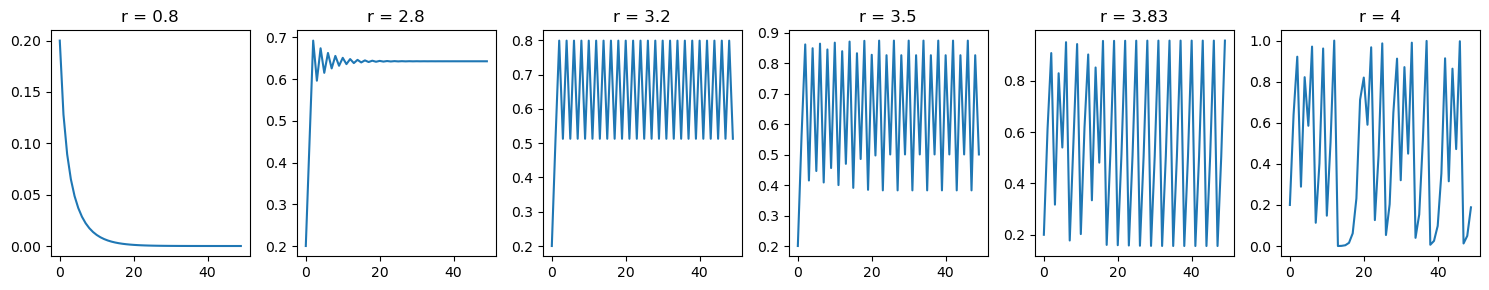
\includegraphics[width=\textwidth]{periodicity.png}
\caption{First fifty iterates from $x_0 = 0.2$ at six parameter values,
showing extinction, alternating convergence to the fixed point, cycles of
period two, four and three, and aperiodic motion.}
\label{fig:periodicity}
\end{figure}

Figure \ref{fig:cobweb} shows the same behaviour geometrically. A cobweb plot
draws the graph of $\logmap$ with the diagonal $y=x$ and traces the
alternating vertical and horizontal segments representing the recursion, so
that fixed points appear as intersections with the diagonal and the local
slope at an intersection is the multiplier. At $r=2$ the orbit reaches the
fixed point in very few steps, which is the superstability of Remark
\ref{rem:superstable} made visible: the graph is flat where it crosses the
diagonal. At $r=3.2$ the cobweb closes into a rectangle, the signature of a
period-two cycle. At $r=4$ it never closes.

\begin{figure}[H]
\centering
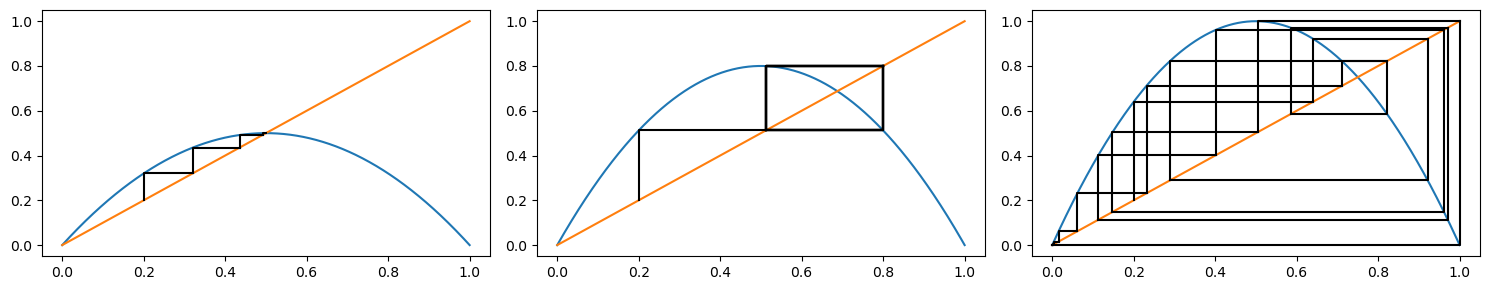
\includegraphics[width=\textwidth]{cobweb.png}
\caption{Cobweb plots at $r=2$, $r=3.2$ and $r=4$. The blue curve is
$\logmap$, the orange line is $y=x$.}
\label{fig:cobweb}
\end{figure}

\subsection{Sensitive dependence}

Two orbits are started from $x_0=0.2$ and $x_0=0.2+10^{-8}$ and their
separation is tracked for fifty iterations at two parameters. Figure
\ref{fig:chaosvis} plots the logarithm of the separation, so an exponential
rate appears as a straight line whose gradient is that rate.

\begin{figure}[H]
\centering
\includegraphics[width=0.62\textwidth]{chaos_vis.png}
\caption{Logarithm of the separation between two orbits started $10^{-8}$
apart, at $r=2.8$ (contracting) and $r=4$ (expanding, then saturating).}
\label{fig:chaosvis}
\end{figure}

Both panels can be checked against results derived above. At $r=2.8$ the
separation contracts, and its decay rate should be $\log|\mu_2| = \log 0.8 =
-0.223$ per iteration by Proposition \ref{prop:stab2}; the observed gradient
is close to that. At $r=4$ the separation grows at a rate close to $\log 2$
per iteration and then saturates at a value of order the diameter of the attractor, beyond which the two orbits
are simply unrelated and the separation stops being meaningful. The saturation
point is itself predictable: starting from $10^{-8}$ and doubling each step,
saturation is expected after $\log(10^{8})/\log 2 \approx 27$ iterations,
which is where it occurs.

\section{The bifurcation diagram}
\label{sec:bifurcation}

For each of $1500$ values of $r$ spanning $[2.5, 4]$, an orbit of $1500$
iterates is generated from $x_0=0.4$, the first $1100$ are discarded as
transient, and the remaining $400$ are plotted above that value of $r$. Where
the attractor is a cycle of period $p$ the points collapse onto $p$ values;
where it is chaotic they fill out bands.

\begin{figure}[H]
\centering
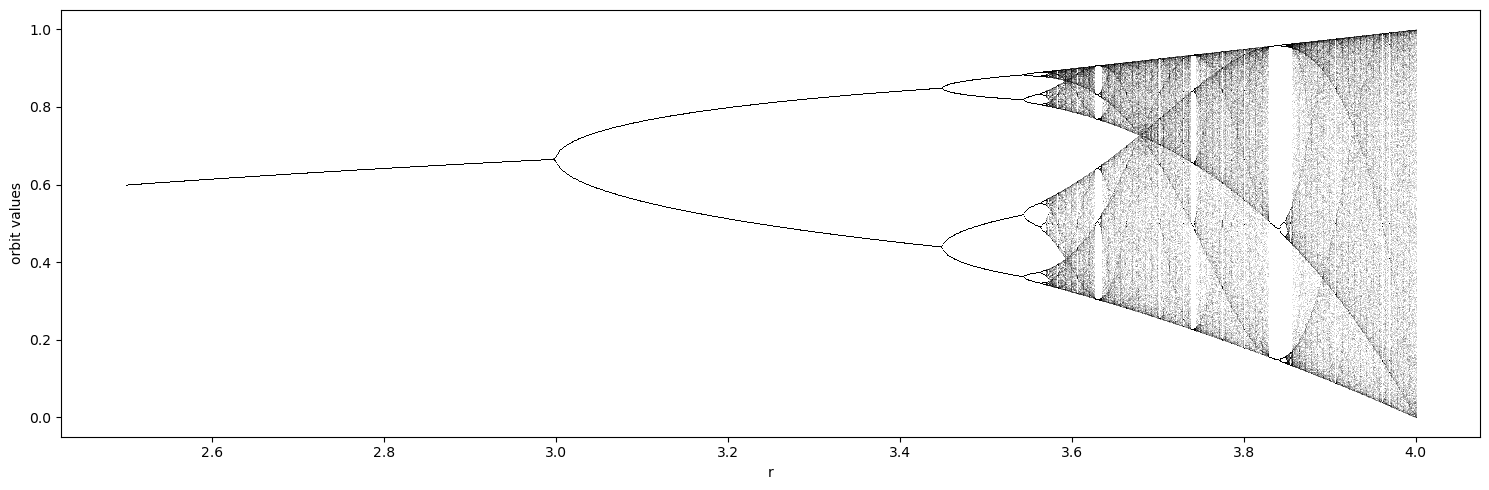
\includegraphics[width=\textwidth]{bifurcation.png}
\caption{Bifurcation diagram over $r\in[2.5,4]$. The single branch splits at
$r=3$, the value derived in Proposition \ref{prop:stab2}.}
\label{fig:bifurcation}
\end{figure}

Two rendering issues materially affected what the diagram shows and were fixed
during the work.

\begin{itemize}
  \item \textbf{Transient contamination.} Too short a transient leaves
    approach trajectories in the plot, appearing as vertical smearing near the
    branch points. This is worst precisely where it is least wanted: near a
    branch point the multiplier approaches $1$ in magnitude and convergence is
    slowest, so the transient requirement is not uniform in $r$ and must be
    set by the worst case rather than the typical one.
  \item \textbf{Overplotting.} With $1500$ parameter values and $400$ iterates
    each, some $600{,}000$ points are drawn, and at ordinary marker sizes the
    periodic branches saturate and become indistinguishable from the chaotic
    bands. The correct marker size and opacity had to be iterated to find, to resolve
    the structure. The points are also accumulated into two flat arrays and
    drawn in a single call rather than plotted per parameter, which is
    substantially faster.
\end{itemize}

The first branch point is known from Proposition \ref{prop:stab2}: the
fixed point loses stability at $r=3$, and the diagram splits there. This is
the last feature that can be checked against a result derived here; beyond it
the branch points are roots of polynomials of rapidly increasing degree, and
locating them is the numerical problem taken up next.

\section{The Feigenbaum constant}
\label{sec:feigenbaum}

\subsection{The quantity}

The cascade consists of parameters $r_1=3<r_2<r_3<\cdots$ at which the
attracting cycle doubles in period. They accumulate at a finite value and the
spacings shrink at an asymptotically constant ratio,
\begin{equation}
  \delta = \lim_{n\to\infty}\frac{r_n-r_{n-1}}{r_{n+1}-r_n} .
  \label{eq:feigdef}
\end{equation}
Feigenbaum's result is that this ratio is identical for a large class of maps
with a quadratic critical point, so it is a property of the mechanism rather
than of the logistic map \cite{Feigenbaum1978}. Its accepted value is quoted
as (C2); the aim here is to recover it independently.

\subsection{Why superstable parameters}

The bifurcation parameters $r_n$ are defined by a cycle multiplier equalling
$-1$. That is numerically awkward: near such a parameter the cycle is only
marginally stable, so orbits converge arbitrarily slowly, and locating the
cycle in order to evaluate its multiplier becomes ill conditioned exactly
where the answer is wanted.

The superstable parameters are a better-conditioned proxy. Define $R_n$ as the
parameter at which the critical point $x=\tfrac12$ is itself a member of the
cycle of period $2^{n}$, that is the root of
\begin{equation}
  g_n(r) := \logmap^{2^{n}}\!\left(\tfrac12\right) - \tfrac12 = 0 .
  \label{eq:superstabledef}
\end{equation}
Each $R_n$ lies strictly between $r_n$ and $r_{n+1}$, so the two sequences
interleave and accumulate at the same point, and the ratio \eqref{eq:feigdef}
computed from either has the same limit. The advantages are concrete: $g_n$ is
evaluated exactly by $2^{n}$ compositions with no iteration to convergence,
the cycle is superstable so no stability computation is involved at all, and
the defining condition is a sign change in a scalar function, which is the
best-conditioned root-finding situation available.

\subsection{Method}

For each period $2^{n}$ up to $256$, the parameter $R_n$ is located in two
stages.

\begin{enumerate}
  \item \textbf{Bracketing.} A bracket $[a,b]$ with $g_n(a)g_n(b)<0$
    containing no other root is required, and this is the principal failure
    mode of the method: $g_n$ has $2^{n}$ roots in the region of interest, and
    bracketing the wrong one yields a value that is internally consistent but
    belongs to a different cycle. The search starts just above the previously
    located parameter and steps upward to the first sign change. The step
    length is the delicate part. A fixed step fails at deeper levels, because
    the spacing between consecutive superstable parameters shrinks by a factor
    of roughly $\delta$ each time, so a step that is safe at period four will
    stride over several roots at period $128$. The step is therefore set
    adaptively to one hundredth of the previous gap, which shrinks at the same
    rate as the structure being resolved.
  \item \textbf{Bisection.} The bracket is halved until its width falls below
    $10^{-12}$, converging to the root. Bisection is chosen as although it
    converges only linearly, it cannot leave its
    bracket, whereas a Newton or secant step on a function with $2^{n}$ nearby
    roots can jump to a neighbouring one with no indication that it has done
    so. 
\end{enumerate}

\subsection{Results}

Successive estimates of the ratio are formed from consecutive triples of
located parameters. Table \ref{tab:feigenbaum} gives them with their absolute
deviation from the quoted value (C2).

\begin{table}[H]
\centering
\begin{tabular}{clll}
\toprule
Deepest period used & Estimate of $\delta$ & Absolute error \\
\midrule
$8$   & $4.708943$ & $3.97\times10^{-2}$ \\
$16$  & $4.680771$ & $1.16\times10^{-2}$ \\
$32$  & $4.662960$ & $6.24\times10^{-3}$ \\
$64$  & $4.668404$ & $7.98\times10^{-4}$ \\
$128$ & $4.668954$ & $2.48\times10^{-4}$ \\
$256$ & $4.669157$ & $4.44\times10^{-5}$ \\
\midrule
Final estimate & $4.669191$ & $1.07\times10^{-5}$ \\
\bottomrule
\end{tabular}
\caption{Successive estimates of the Feigenbaum ratio from the located
superstable parameters, against the published value
$\delta = 4.669\,201\,609\,102\,99$.}
\label{tab:feigenbaum}
\end{table}

The final estimate is $4.669191$ against $4.669202$, agreeing to five
significant figures. The error falls by roughly a factor of four or five per
level, which is consistent with the leading correction to \eqref{eq:feigdef}
itself decaying geometrically in the level index, though the sequence is not
smooth enough at these depths to claim that as a measured rate.

\subsection{Why the cascade cannot be followed further}

Two effects limit the computation and pull in the same direction. The spacings
$R_n-R_{n-1}$ shrink by a factor of about $4.67$ per level, so by period $256$
the differences entering \eqref{eq:feigdef} are of order $10^{-7}$ and the
subtraction is losing significance rapidly in double precision. At the same
time the number of compositions needed to evaluate $g_n$ doubles at each
level, and each composition contributes rounding error that is itself
amplified along the orbit by the derivative of the map. Five significant
figures is close to what this route supports in double precision; going
further is a question of extended-precision arithmetic rather than of a better
algorithm.

\section{The Lyapunov exponent}
\label{sec:lyapunov}

\subsection{Definition and estimator}

The Lyapunov exponent measures the average exponential rate at which nearby
orbits separate. Linearising along an orbit, a displacement $\delta x_0$
evolves to $\delta x_n=\delta x_0\prod_{k=0}^{n-1}\logmap'(x_k)$, so the mean
growth rate per step is
\begin{equation}
  \lambda = \lim_{N\to\infty}\frac{1}{N}\sum_{n=0}^{N-1}\log\bigl|\logmap'(x_n)\bigr| ,
  \label{eq:lyapunov}
\end{equation}
a time average of $\log|\logmap'|$ along the orbit. A positive value means
exponential separation and hence chaos; a negative value means contraction
onto an attracting cycle. The estimator is \eqref{eq:lyapunov} evaluated over
an orbit of $100{,}000$ iterates at $r=4$ from $x_0=0.2$.


\subsection{Result}

At $r=4$ the exact value is $\log2 = 0.6931472$ by (C1). The measured value is
\begin{equation}
  \lambda_{\text{measured}} = 0.6931444 ,
\end{equation}
a relative difference of $4.0\times10^{-6}$, or $0.0004$\%. Since the
sum in \eqref{eq:lyapunov} is an average of weakly correlated terms, a
residual of this size is consistent with the statistical error of a
finite-length average rather than with any systematic defect. The measurement
also confirms, after the fact, the growth rate observed in Figure
\ref{fig:chaosvis} and the saturation estimate made from it.

\section{The invariant density at $r=4$}
\label{sec:density}

\subsection{What is being computed}

Section \ref{sec:orbits} established that individual orbits at $r=4$ are not
computable beyond a few dozen steps. The object that is computable, and
reproducible, is the distribution of the orbit over the interval. A density
$\rho$ is \emph{invariant} if a population of initial points distributed
according to $\rho$ remains so distributed after one application of the map.
Formally $\rho$ is a fixed point of the transfer operator, also called the
Perron-Frobenius operator,
\begin{equation}
  (\PF\rho)(y) = \sum_{x\,:\,\logmap(x)=y}\frac{\rho(x)}{|\logmap'(x)|} ,
  \label{eq:transferoperator}
\end{equation}
which pushes a density forward one step: each preimage contributes its own
density, weighted by the reciprocal of the local stretching factor, since a
region that is stretched has its density diluted. An invariant density
satisfies $\PF\rho=\rho$.

At $r=4$ that density is the arcsine density \eqref{eq:arcsine}, quoted as
(C1). It is strongly non-uniform, diverging at both endpoints, so a typical
orbit spends disproportionately much of its time near $0$ and $1$. The
divergences are integrable and $\int_0^1\rho=1$ as required.

\subsection{Estimation}

Four independent orbits of $100{,}000$ iterates are generated from four random
starting points and each is histogrammed into $200$ equal bins. Figure
\ref{fig:histogram} overlays each histogram with \eqref{eq:arcsine}.

\begin{figure}[H]
\centering
\includegraphics[width=\textwidth]{histogram_vs_arcsin.png}
\caption{Histograms of four independent orbits at $r=4$, each of $100{,}000$
iterates from a random start, overlaid with the arcsine density.}
\label{fig:histogram}
\end{figure}

Using four different starting points rather than one is what justifies the
word invariant: the four histograms are visually indistinguishable, and their
agreement with the closed form is quantified in Table \ref{tab:density}. This
is also the practical evidence for  Section \ref{sec:orbits} that the
statistics do not depend on which particular orbit is followed, despite the
individual orbits being pointwise unrelated to one another after a few dozen
steps.

\begin{table}[H]
\centering
\begin{tabular}{cl}
\toprule
Orbit & Mean absolute difference from \eqref{eq:arcsine} \\
\midrule
$1$ & $0.0287$ \\
$2$ & $0.0288$ \\
$3$ & $0.0311$ \\
$4$ & $0.0331$ \\
\bottomrule
\end{tabular}
\caption{Agreement between each histogram and the arcsine density, measured
over the central $80\%$ of the interval.}
\label{tab:density}
\end{table}

Three points required correction during the work, and each is a general point
about comparing an empirical histogram with a continuous density rather than
anything specific to this map.

\begin{itemize}
  \item \textbf{Normalisation.} Raw counts must be divided by the number of
    samples and the bin width, not by the number of samples alone, to be
    comparable with a density. Dividing by the sample count alone gives a
    probability mass per bin, which depends on the bin width and does not
    converge to $\rho$ as the bins are refined.
  \item \textbf{Bin-centre alignment.} The comparison must evaluate $\rho$ at
    bin centres, obtained by averaging consecutive bin edges, rather than at
    the edges themselves. A half-bin offset is visually negligible in the flat
    central region but conspicuous near the endpoints where $\rho$ varies
    rapidly, and it does not shrink under refinement as quickly as one might
    expect, because the error is proportional to $\Delta\rho'$ and $\rho'$
    diverges.
  \item \textbf{Domain of the error.} The error was originally accumulated
    over the full interval, including the end bins where $\rho$ diverges.
    Those bins dominate any norm, and the resulting number measures the
    singularity rather than the quality of the estimate. All errors reported
    here therefore use the central $80\%$ of the interval, bins $20$ to $180$
    of $200$, and the same convention is carried into Section \ref{sec:ulam}
    so that the two are directly comparable.
\end{itemize}

\subsection{What this does and does not establish}

The agreement shows that a single orbit, pointwise meaningless after a few
dozen steps, nonetheless samples the invariant measure accurately, and that
four different orbits sample the same one. It does not constitute a
computation of the invariant density from the map: the arcsine form was quoted
rather than derived, and the orbits were used only to sample it. Obtaining the
density from the map itself, without knowing the answer in advance, requires
discretising the operator \eqref{eq:transferoperator}. That is the subject of
the next section, and it is where the project stops checking against a known
answer and starts producing one.

\section{Coarse-graining into a Markov chain: Ulam's method}
\label{sec:ulam}

\subsection{The idea}

Ulam's method replaces the transfer operator \eqref{eq:transferoperator},
which acts on an infinite-dimensional space of densities, with a finite matrix
\cite{Ulam1960,Li1976}. Partition $[0,1]$ into $N$ equal boxes
$I_1,\ldots,I_N$ and set
\begin{equation}
  P_{ij} = \frac{m\bigl(I_i\cap\logmap^{-1}(I_j)\bigr)}{m(I_i)} ,
  \label{eq:ulam}
\end{equation}
the fraction of box $i$ that lands in box $j$. Each row sums to one, so $P$ is
a stochastic matrix and the deterministic map has been coarse-grained into a
Markov chain on $N$ states: the position within a box is discarded, and what
survives is the transition probability between boxes. The discretised
invariant density is then the stationary distribution $\pi$ with $\pi P=\pi$.

This is the conceptual centre of the project. A system containing no
randomness has been turned into a probabilistic object, and the
information discarded is the resolution within a box. What makes it
work is that the map is expanding: a box is stretched across several boxes at
each step, so the coarse-grained description is not merely a lossy summary but
approaches the right answer as the boxes shrink.

\subsection{Building the matrix exactly from the map}

At $r=4$ the preimage of a point has two closed-form branches,
\begin{equation}
  f_4^{-1}(y) = \left\{\frac{1-\sqrt{1-y}}{2},\ \frac{1+\sqrt{1-y}}{2}\right\} ,
  \label{eq:preimages}
\end{equation}
so the preimage of a box $I_j$ is a union of two intervals obtained by
applying \eqref{eq:preimages} to its endpoints. Note that the left branch is
decreasing in $y$ and the right branch increasing, so the two preimage
intervals must be assembled with their endpoints in the correct order. For
each box $I_i$ the overlap with each of those two intervals is computed
directly, and dividing by the box width $1/N$ converts a length into a
probability. This evaluates \eqref{eq:ulam} exactly, by interval arithmetic,
with no orbit and no sampling anywhere in the construction.

The stochasticity of $P$ is not imposed but is a consequence of the two
branches covering the whole interval, so checking it is a real test of the
construction rather than a formality. The largest deviation of a row sum from
one is $2.1\times10^{-14}$, consistent with accumulated rounding alone.

The importance of building the matrix this way is that the resulting
stationary distribution is a discretisation of the operator, so its
agreement with the arcsine density is independent confirmation, rather than a
restatement of the histogram of Section \ref{sec:density}.

\subsection{Power iteration}

The stationary distribution is computed by a power iteration written directly
rather than by calling a library eigensolver, since the numerical method is
the point of the exercise. From a probability vector $v_0$,
\begin{equation}
  v_{k+1} = \frac{v_k P}{\|v_k P\|_1} ,
  \label{eq:power}
\end{equation}
iterated until the $\ell^1$ change between successive vectors falls below
$10^{-10}$, subject to a cap of $2000$ iterations after which failure is
reported rather than a partially converged vector returned. Renormalising at
each step is not strictly necessary for a stochastic matrix, whose action
preserves the total mass, but it prevents rounding drift from accumulating
over hundreds of iterations.

Convergence of this iteration to the dominant left eigenvector, and the
uniqueness of the stationary distribution, are properties of the chain rather
than assumptions, and are worth testing rather than taking on trust. The
iteration was therefore run from two deliberately dissimilar starting vectors,
the uniform distribution and a random draw from a Dirichlet distribution, and
the two limits agree to within $10^{-8}$ in $\ell^1$. Figure
\ref{fig:powerconv} plots the logarithm of the successive change for both. The
two traces are close to straight lines of the same gradient, which is the
expected behaviour: the convergence rate of a power iteration is set by the
ratio of the second largest eigenvalue modulus to the first, a property of the
matrix and not of where the iteration started. Both reach the tolerance in
under forty iterations.

\begin{figure}[H]
\centering
\includegraphics[width=0.62\textwidth]{covergence.png}
\caption{Logarithm of the $\ell^1$ change per power iteration, from a uniform
start (left) and a random Dirichlet start (right), with $N=200$.}
\label{fig:powerconv}
\end{figure}

\subsection{The second construction, and why it is kept}

The same method can be applied with the matrix estimated from data instead of
derived from the map: run a single orbit of $M=100{,}000$ points, count the
transitions between boxes, and normalise the rows. This is the more obvious
construction, and it is the one implemented first.

It contains no new information. Its stationary distribution reproduces the
orbit's own occupancy histogram to a maximum absolute difference of
$9.7\times10^{-6}$, which is the diagnostic that identifies the problem: what
is being recovered is the Section \ref{sec:density} histogram, arrived at by a
longer route. The matrix has $N^2$ entries estimated from a fixed number of
observed transitions, so refining the partition does not refine the estimate,
it thins the data.

Figure \ref{fig:stationary} shows both stationary densities against the closed
form at $N=200$. Both track it well; the map-based one has visible steps near
the left endpoint, where the box width is too coarse to resolve a diverging
density. The mean absolute difference between the map-based stationary density
and the closed form, over the same central $80\%$ used in Section
\ref{sec:density}, is $0.0331$, which is comparable to the histogram errors in
Table \ref{tab:density} despite having been obtained without generating a
single orbit.

\begin{figure}[H]
\centering
\includegraphics[width=\textwidth]{stationary_Density.png}
\caption{Arcsine closed form against the two stationary densities at $N=200$,
one from the exactly constructed matrix and one from the matrix counted off a
single orbit.}
\label{fig:stationary}
\end{figure}

\subsection{Behaviour under refinement}

For box counts from $N=50$ to $N=1600$, spaced geometrically at roughly
$\sqrt2$ per step, the whole pipeline is run at each $N$: build the matrix,
power-iterate to the stationary distribution, convert it to a density by
multiplying by $N$, and compare against the arcsine formula over the central
$80\%$ of the interval. The error is the mean absolute difference, and both
axes are logarithmic so that a power law appears as a straight line whose
gradient is the exponent.

\begin{figure}[H]
\centering
\includegraphics[width=0.72\textwidth]{final.png}
\caption{Error against the arcsine density as a function of box count, for the
matrix built exactly from the map (circles) and estimated from a single orbit
of $100{,}000$ points (squares), with the $\sqrt{N/M}$ sampling reference
shown dashed.}
\label{fig:refinement}
\end{figure}

\begin{table}[H]
\centering
\begin{tabular}{lll}
\toprule
Construction of $P$ & Fitted gradient & Interpretation \\
\midrule
Exact, from the map & $-0.51$ & error falls as boxes shrink \\
Estimated, from one orbit & $+0.55$ & error rises as data per box thins \\
\bottomrule
\end{tabular}
\caption{Gradient of $\log(\text{error})$ against $\log N$ over $N=50$ to
$1600$, for the two constructions.}
\label{tab:ulamslopes}
\end{table}

The map-based curve decreases at a trend of roughly $N^{-1/2}$ over this
range. The trend is not perfectly clean: two of the refinement steps tick
upward before the decrease resumes, so this is best described as an
approximate rate rather than as a measured convergence order, and therefore
no claim is made about the asymptotic order.

The orbit-based curve increases, at almost exactly the mirrored gradient. The
dashed reference is $\sqrt{N/M}$, the expected scaling of sampling error when
$M$ fixed observations are spread across $N$ boxes, and the measured points
lie along it. That agreement is what identifies the cause as sampling noise
rather than a defect in the method, and it is why the two constructions were
worth running side by side: without the reference line, a rising error curve
looks like a broken implementation.

The two curves answer different questions. Does the method converge, and does
this estimate of it converge? The answers are opposite, and the distinction
between them is the point. Refining a discretisation helps only if what is
being refined is the operator; refining an estimator built from a fixed
quantity of data makes it worse, and the two are easy to conflate when both
are described as Ulam's method.

\section{Conclusion}

Analytically, this project derives the parameter range $0\le r\le4$ for which
the unit interval is preserved, locates both fixed points, derives their
multipliers and hence the exact stability ranges $0\le r<1$ and $1<r<3$, and
identifies the transcritical and period-doubling bifurcations at $r=1$ and
$r=3$. Both the fixed-point location and the multiplier are then confirmed
numerically across one hundred randomly drawn parameters.

Numerically, it produces the bifurcation diagram with the derived branch point
$r=3$ reproduced; recovers the Feigenbaum constant as $4.669191$ against the
published $4.669202$, agreeing to five significant figures, by locating
superstable parameters with an adaptively bracketed bisection, and identifies
the precision limit that prevents the cascade being followed further; computes
the Lyapunov exponent at $r=4$ as $0.6931444$ against the exact
$\log2 = 0.6931472$; and estimates the invariant density from four independent
orbits, matching the arcsine closed form once the normalisation, alignment and
error-domain issues are corrected.

Finally it coarse-grains the map into a Markov chain by Ulam's method,
building the transition matrix exactly from the two preimage branches at
$r=4$, solving for the stationary distribution by a power iteration written
from scratch and verified to be independent of its starting vector, and
measuring the behaviour of the error under refinement of the partition. Built
from the map, the error falls at a trend of about $N^{-1/2}$; built from a
single trajectory, it rises along $\sqrt{N/M}$.

\appendix

\section{Summary of validation}

\begin{table}[H]
\centering
\small
\begin{tabular}{p{4.3cm}p{4.3cm}p{4.6cm}}
\toprule
Computation & Reference quantity & Source of reference \\
\midrule
Attained fixed point, $100$ random $r$ & $1-1/r$ & Derived, Prop.\ \ref{prop:fixed} \\
Measured multiplier, $100$ random $r$ & $2-r$ & Derived, Prop.\ \ref{prop:stab2} \\
Orbit decay rate at $r=2.8$ & $\log 0.8 = -0.223$ & Derived, Prop.\ \ref{prop:stab2} \\
First branch point & $r=3$ & Derived, Prop.\ \ref{prop:stab2} \\
Cobweb behaviour at $r=2$ & Superstability, $\mu_2=0$ & Derived, Remark \ref{rem:superstable} \\
Feigenbaum ratio & $4.669\,201\,609\ldots$ & Cited, (C2) \\
Lyapunov exponent at $r=4$ & $\log 2$ & Cited, (C1) \\
Orbit separation saturation & $\log(10^8)/\log 2 \approx 27$ steps & Derived from (C1) \\
Invariant density, four orbits & Arcsine density & Cited, (C1) \\
Ulam row sums & Exactly $1$ & Stochasticity of $P$ \\
Power iteration limit & Independent of start vector & Uniqueness of $\pi$ \\
Orbit-based stationary vector & Orbit occupancy histogram & Diagnostic, Sec.\ \ref{sec:ulam} \\
Orbit-based error growth & $\sqrt{N/M}$ & Sampling argument \\
\bottomrule
\end{tabular}
\caption{Every result in this document and the independent quantity against
which it is checked.}
\label{tab:validation}
\end{table}

\section{Computational environment}

All computations were performed in Python 3 with NumPy in IEEE double
precision, and figures produced in Matplotlib. The companion notebook is
\texttt{chaos\_prob.ipynb}.

\begin{thebibliography}{9}

\bibitem{May1976}
R.~M. May.
\newblock Simple mathematical models with very complicated dynamics.
\newblock \emph{Nature}, 261:459--467, 1976.

\bibitem{Feigenbaum1978}
M.~J. Feigenbaum.
\newblock Quantitative universality for a class of nonlinear transformations.
\newblock \emph{Journal of Statistical Physics}, 19(1):25--52, 1978.

\bibitem{Strogatz2015}
S.~H. Strogatz.
\newblock \emph{Nonlinear Dynamics and Chaos}.
\newblock Westview Press, 2nd edition, 2015.

\bibitem{Devaney2003}
R.~L. Devaney.
\newblock \emph{An Introduction to Chaotic Dynamical Systems}.
\newblock Westview Press, 2nd edition, 2003.

\bibitem{Ott2002}
E.~Ott.
\newblock \emph{Chaos in Dynamical Systems}.
\newblock Cambridge University Press, 2nd edition, 2002.

\bibitem{Ulam1960}
S.~M. Ulam.
\newblock \emph{A Collection of Mathematical Problems}.
\newblock Interscience, 1960.

\bibitem{Li1976}
T.-Y. Li.
\newblock Finite approximation for the Frobenius-Perron operator: a solution to
  Ulam's conjecture.
\newblock \emph{Journal of Approximation Theory}, 17(2):177--186, 1976.

\bibitem{BoyarskyGora1997}
A.~Boyarsky and P.~G\'{o}ra.
\newblock \emph{Laws of Chaos: Invariant Measures and Dynamical Systems in One
  Dimension}.
\newblock Birkh\"{a}user, 1997.

\end{thebibliography}

\end{document}
